\documentclass[compress]{beamer}

\usepackage[utf8]{vntex}
\usepackage{longtable}
\usepackage{amsmath}
\usepackage{amsmath}
\usepackage{amsfonts}
\usepackage{cases}
\usepackage{amssymb}
\usepackage[utf8]{inputenc}
\usepackage[absolute,overlay]{textpos}
\usepackage{listings}

\lstset{
	language = Java,
	frame = single,
	tabsize = 3
}

\usetheme{Warsaw}
%\usetheme{Antibes}
%\usecolortheme{spruce}
%\setbeamercolor{structure}{fg=cyan!90!blue}
%\newtheorem{theorem}{Định lý}[]

\expandafter\def\expandafter\insertshorttitle\expandafter{%
    \insertshorttitle\hfill%
    \insertframenumber\,/\,\inserttotalframenumber}
      
\AtBeginSection[] % Do nothing for \section*
{
\begin{frame}
\tableofcontents[currentsection]
\end{frame}
}
\AtBeginSubsection[] % Do nothing for \section*
{
\begin{frame}
\tableofcontents[currentsection, currentsubsection]
\end{frame}
}

\title[Lập kế hoạch di chuyển cho robot]{Lập kế hoạch di chuyển cho robot} 

\author[Nguyễn Tuấn Đạt, Đặng Quang Trung, Phan Anh Tú (SoICT)]{
Sinh viên thực hiện\\
Nguyễn Tuấn Đạt - 20130856 \\
Phan Anh Tú - 20134501 \\
Đặng Quang Trung - 20134145 \\[1em]
Giảng viên \\
PGS.TS Huỳnh Thị Thanh Bình}

\begin{document}

\begin{frame}[plain]
\titlepage
\end{frame}

\begin{frame}[plain]{Nội dung trình bày}
\tableofcontents
\end{frame}

\section{Giới thiệu bài toán}

\subsection{Không gian làm việc, không gian cấu hình}
\begin{frame}{Giới thiệu bài toán}
\begin{itemize}
\item $\mathcal{R}$ là robot di chuyển trong không gian 2 chiều (không gian làm việc) 
\item $S = \{\mathcal{P}_1, ...., \mathcal{P}_t\}$ các chướng ngại vật 
\item Ký hiệu $\mathcal{R}(x,y)$ đại diện cho vector vị trí các đỉnh của robot
\item Robot có các đỉnh: $(1,-1), (1,1), (0,3), (-1,1), (-1,-1)$ => $\mathcal{R}(6,4) = (7,3), (7,5), (6,7), (5,5), (5,3)$
\begin{figure}[H]
\centering
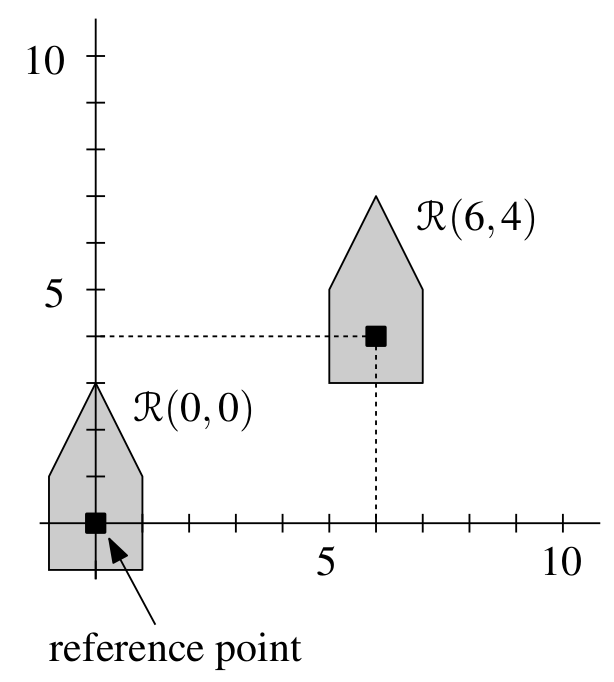
\includegraphics[scale=0.2]{work_space_definition.png}
\end{figure}
\end{itemize}
\end{frame}

\begin{frame}{Giới thiệu bài toán}
\begin{itemize}
\item Định nghĩa thêm một tham số ($\phi$) để biểu diễn hướng của robot
\item Ký hiệu $\mathcal{R}(x,y,\phi)$ xác định vị trí và hướng của robot
\begin{figure}[H]
\centering
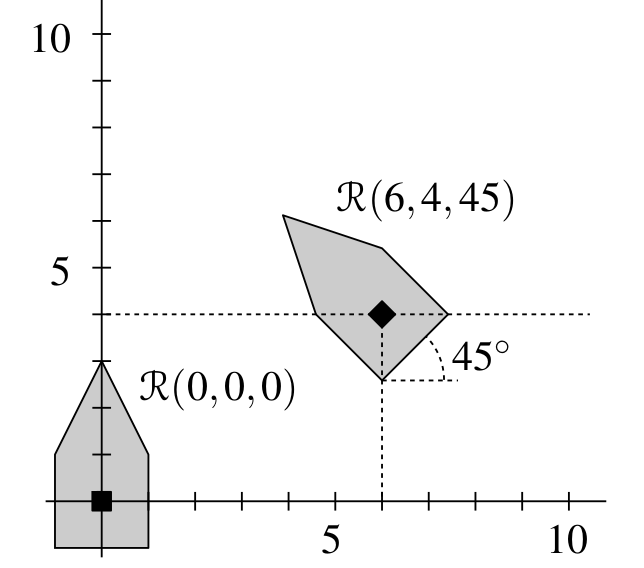
\includegraphics[scale=0.2]{work_space_with_rotate.png}
\end{figure}
\item Không gian các tham số thường được gọi là không gian cấu hình ($\mathcal{C}(\mathcal{R})$). 
\item Điểm $(x,y,\phi)$ trong không gian cấu hình sẽ tương ứng với vị trí $\mathcal{R}(c,y,\phi)$ trong không gian làm việc.
\end{itemize}
\end{frame}

\begin{frame}{Giới thiệu bài toán}
\begin{itemize}
\item Không gian làm việc là không gian thực tế mà robot di chuyển 
\item Không gian cấu hình là không gian các tham số của robot (điểm tham chiếu, hướng của robot)
\item Một đa giác (hình của robot) trong không gian làm việc sẽ được biểu diễn bởi một điểm trong không gian cấu hình 
\item Mọi điểm trong không gian cấu hình tương ứng với một vài vị trí thực của robot trong không gian làm việc
\item Một đường đi của robot trong không gian làm việc sẽ tương đương với một đường cong trong không gian cấu hình
\begin{figure}[H]
\centering
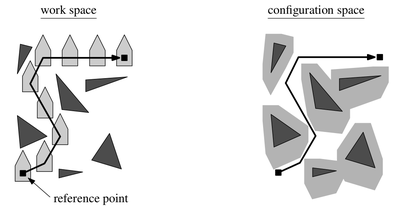
\includegraphics[scale=0.45]{path.png}
\end{figure}
\end{itemize}
\end{frame}


\section{Lập kế hoạch di chuyển}
\subsection{Bản đồ hình thang}
\begin{frame}{Bản đồ hình thang}
\begin{itemize}
\item Xét một vùng kín $B$, bên trong gồm các chướng ngại vật có dạng đa giác. 
\begin{figure}[H]
\centering
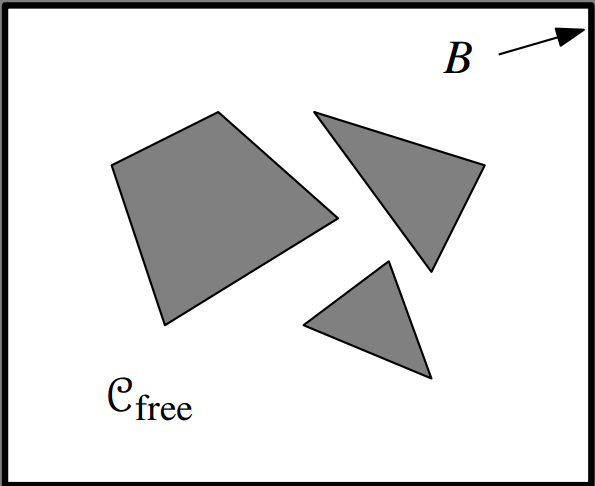
\includegraphics[scale=0.2]{normal.png}
\end{figure}
\item Xây dựng tập $S$ là tập các cạnh của các đa giác chướng ngại vật.
\item Hai cạnh bất kì phải là non-crossing tức là chúng không giao nhau hoặc có duy nhất một điểm mút chung.
\item Hai điểm mút bất kì của hai cạnh bất kì là không cùng tọa độ x.
\end{itemize}
\end{frame}

\begin{frame}{Bản đồ hình thang}
\begin{itemize}
\item Từ mỗi đầu mút của một đoạn thẳng trong $S$, vẽ một đường đi xuống một đường đi lên. 
\item Hai đường thẳng này sẽ dừng lại khi gặp một đoạn thẳng khác hoặc biên của miền bao phủ ($B$).
\begin{figure}[H]
\centering
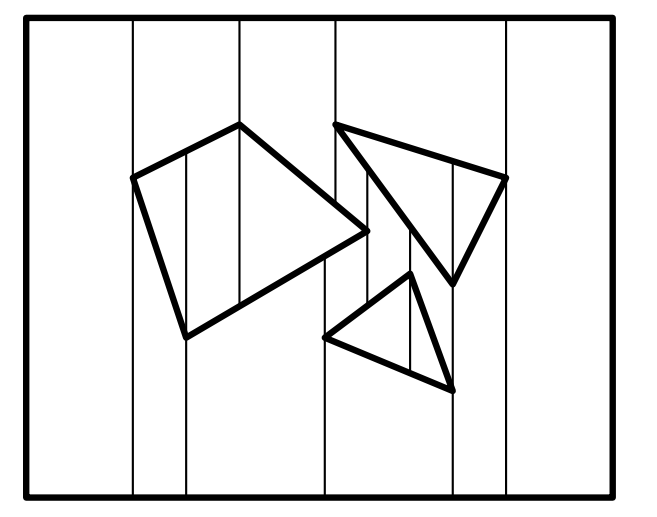
\includegraphics[scale=0.2]{trmap.png}
\end{figure}
\end{itemize}
\end{frame}

\subsection{Lập kế hoạch di chuyển}
\begin{frame}{Lập kế hoạch di chuyển}
\textbf{Algorithm} \textsc{ComputeFreeSpace(S)}\\
\emph{Input}. Tập các chướng ngại vật $S$\\
\emph{Output}. Bản đồ hình thang của không gian trống\\
1. $E$ tập các cạnh của của các chướng ngại vật trong $S$\\
2. Xây dựng bản đồ hình thang $\mathcal{T}(E)$\\
3. Xóa bỏ các hình thang mà cạnh của nó ở bên trong một trong những chướng ngại vật
\begin{figure}[H]
\centering
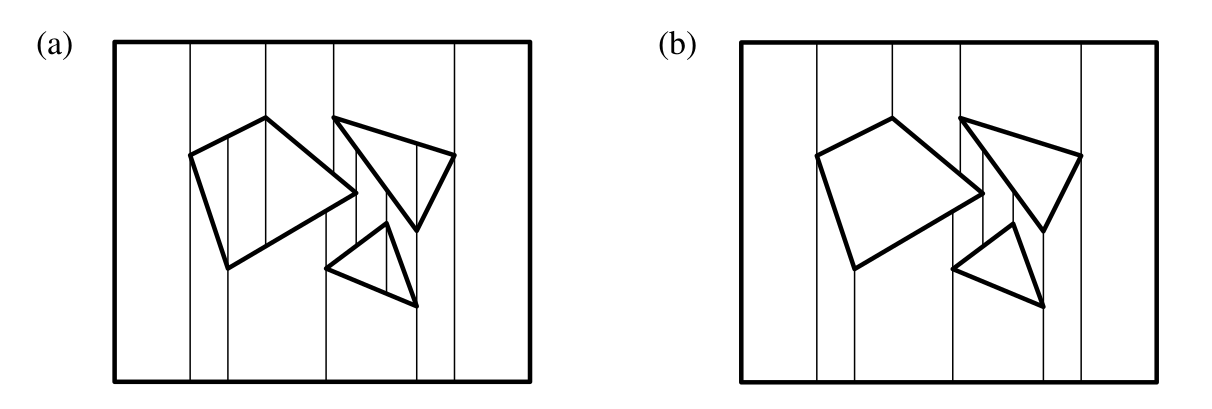
\includegraphics[scale=0.25]{trapezoidal_free_space.png}
\end{figure}
\end{frame}

\begin{frame}{Lập kế hoạch di chuyển}
Xây dựng \emph{road map} ($\mathcal{G}_{road}$) trên không gian trống. 
\begin{itemize}
\item Với mỗi hình thang trong bản đồ hình thang, xác định tâm và trung điểm các cạnh đáy của nó. 
\item Các điểm đó sẽ là tập các nút của đồ thị.
\item Một cạnh được nối giữa một nút là tâm và một nút là trung điểm của cạnh đáy của cùng một hình thang
\end{itemize}
\begin{figure}[H]
\centering
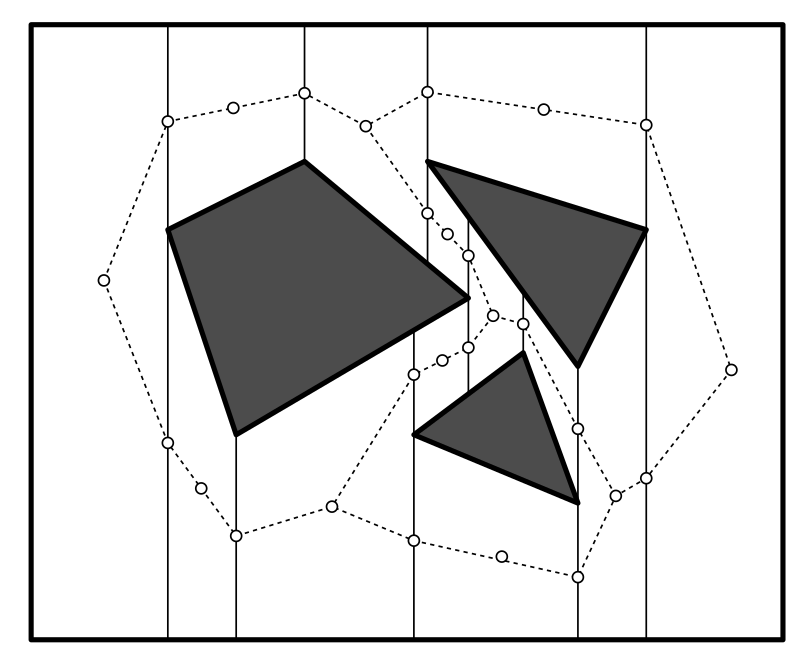
\includegraphics[scale=0.2]{road_map.png}
\end{figure}
\end{frame}

\begin{frame}{Lập kế hoạch di chuyển}
Cần xây dựng đường đi từ $p_{start}$ đến điểm $p_{end}$ sử dụng bản đồ hình thang $\mathcal{T}(\mathcal{C}_{free})$
\begin{itemize}
\item Nếu $p_{start}$ và $p_{goal}$ ở cùng trong một hình thang thì ta chỉ việc nối 2 điểm đó là có đường đi của robot.
\item Nếu $p_{start}$ và $p_{goal}$ ở 2 hình thang khác nhau
\begin{itemize}
\item Xác định các hình thang $\Delta_{start}$ và $\Delta_{goal}$ chứa các điểm $p_{start}$ và $p_{goal}$
\item Xác định các điểm $v_{start}$ (tâm của hình thang $\Delta_{start}$) và $v_{goal}$ (tâm của hình thang $\Delta_{goal}$) là các nút trên đồ thị $\mathcal{G}_{road}$
\item Nối các điểm $p_{start}$ với $v_{start}$, $p_{goal}$ với $v_{goal}$
\item Tìm đường đi từ $v_{start}$ tới $v_{goal}$ ta có đường đi từ $p_{start}$ tới $p_{goal}$
\end{itemize}
\end{itemize}
\end{frame}



\begin{frame}[plain]{Thank you for attention! Any Question?}
Hope you enjoy!
\end{frame}

\end{document}
